\documentclass[usenames,dvipsnames,aspectratio=1610]{beamer}

\setbeamertemplate{nagivation symbols}{}
%%% Standard includes
\usepackage{amsthm, amssymb, amsmath, hyperref, xypic}
\usepackage{lmodern,subfig,multicol}

\usetheme[sectionpage=none]{metropolis}

%%% Graphics 
\usepackage{tikz}
\usetikzlibrary{shapes,arrows.meta,decorations.markings}
%\usepackage[all]{xy}
%\usepackage{graphicx}
%\usepackage{subcaption}


%%% Margins, formatting
%\usepackage{fullpage}
%\usepackage[margin=1in]{geometry}
\usepackage{setspace}
\usepackage{fancyhdr,lastpage}
%\usepackage{afterpage}
%\pagenumbering{gobble}
%\addtolength{\textwidth}{4cm}
%\addtolength{\hoffset}{-2cm}
%\addtolength{\textheight}{3.5cm}
%\addtolength{\voffset}{-2.5cm}
%\fancyhead{}
%\doublespacing
\usepackage{enumitem}
%\setitemize{noitemsep}
%\linespacing{1.1em}


%% Define the headers and footers for the first page, call it 'first'
%\fancypagestyle{first}{%
  %\renewcommand{\headrulewidth}{0pt}
%\fancyfoot[C]{\thepage~of~\pageref{LastPage}}
%\renewcommand{\footrulewidth}{0pt}}

%\usepackage{multicol}

%%% Bibliography
%\usepackage[
%backend=bibtex,
%style=numeric,
%block=space
%]{biblatex}
%\addbibresource{refs.bib}
%\renewbibmacro{in:}{}
%\DeclareNameAlias{sortname}{first-last}

%%% Fonts
%\usepackage{helvet}
%\usepackage{anyfontsize,libertine}
%\usepackage{libertinust1math}
%\usepackage[T1]{fontenc}
%\usepackage{mathpazo}
%\usepackage{eulervm}
%\renewcommand{\familydefault}{\sfdefault}


% Quiet beamer complaints
\renewcommand\textbullet{\ensuremath{\bullet}}



%%% New commands

\newcommand{\Mdef}[2]{\newcommand{#1}{\relax \ifmmode #2 \else $#2$\fi}}

%% thereoms, prop, etc
%\newtheorem{theorem}{Theorem}
%\newtheorem{lemma}[theorem]{Lemma}
%\newtheorem{prop}[theorem]{Proposition}
%\newtheorem{definition}[theorem]{Definition}
%\newtheorem{corollary}[theorem]{Corollary}
%\newtheorem{example}[theorem]{Example}
%\newtheorem{remark}[theorem]{Remark}
%\newtheorem{conjecture}[theorem]{Conjecture}
%\newtheorem*{question}{Question}
%\newtheorem*{questions}{Questions}

%% operators
\DeclareMathOperator{\Hom}{Hom}
\DeclareMathOperator{\cok}{cok}
\DeclareMathOperator{\im}{im}
\DeclareMathOperator{\id}{id}

%% Letters
\Mdef{\SA}{\mathcal{A}}
\Mdef{\SAD}{\mathcal{A}_*}
\Mdef{\SAS}{\mathrm{Sq}}
\Mdef{\SAP}{\mathcal{P}}

\Mdef{\B}{B}
\Mdef{\F}{\mathbb{F}}
\Mdef{\M}{\mathcal{M}}
\Mdef{\N}{\mathbb{N}}
\Mdef{\R}{\mathbb{R}}
\Mdef{\Z}{\mathbb{Z}}
\Mdef{\Q}{\mathbb{Q}}
\Mdef{\vectk}{\mathrm{vect}_k}

\newcommand{\Fp}[1]{\mathbb{F}_{#1}}
\newcommand{\HPM}[1]{H_{#1}^{\mathrm{MP}}(f;\mathbb{F}_2)}


%% arrows
\newcommand{\ra}{\rightarrow}
\newcommand{\lra}{\longrightarrow}
\newcommand{\la}{\leftarrow}
\newcommand{\lla}{\longleftarrow}

%% symbols
\newcommand{\tensor}{\otimes}
\newcommand{\dsum}{\oplus}
\newcommand{\Dsum}{\bigoplus}
\newcommand{\susp}{\Sigma}



\tikzstyle{decision} = [diamond, draw, fill=blue!20, 
    text width=4.5em, text badly centered, node distance=3cm, inner sep=0pt]
\tikzstyle{block} = [rectangle, draw, fill=blue!20, 
    text width=5em, text centered, rounded corners, minimum height=4em]
\tikzstyle{wideblock} = [rectangle, draw, fill=blue!20, 
    text width=7em, text centered, rounded corners, minimum height=4em]
%\tikzstyle{line} = [draw, -latex']
\tikzstyle{line} = [draw, -Latex]
\tikzstyle{cloud} = [draw, ellipse,fill=red!20, node distance=3cm,
    minimum height=2em]
%%%%%%%%%%%%%%%%%%%%%%%%


\title{An Introduction to Topological Data Analysis}
\author{Michael Catanzaro}
\date{NCS MAA Fall 2018 \\ Southwest Minnesota State University}
\institute{Iowa State University}

\begin{document}
\setbeamercolor{background canvas}{bg=white}
\begin{frame}[plain]
  \maketitle
\end{frame}

\metroset{block=fill}

\begin{frame}
  \frametitle{Algebraic Topology}
  \begin{block}{What is algebraic topology?}
    Topology is a branch of mathematics which is good at extracting global
    qualitative features from complicated geometric structures. 
    
    Algebraic topology provides a set of {\em algebraic} descriptors to topological objects.
  \end{block}

  \begin{block}{Questions and scope}
    Topological questions surround different notions of connectedness:
    connected components, loops, voids, etc.

    Two topological spaces are equivalent through the lens of topology if one
    can be {\em continuously} deformed to the other.
  \end{block}

 show some examples
\end{frame}

\begin{frame}{Invariants of topological spaces}
  Algebraic Topology assigns {\em invariants} to topological spaces.

  If two spaces are the same, then the invariants must be the same.

  If the invariants are not the same, then the two spaces are not the same.
\end{frame}

\begin{frame}{Topological Data Analysis}

  \begin{alertblock}{Goal}
    {\bf Topological data analysis uses topology to summarize and study the
    `shape' of data.}
  \end{alertblock}
\end{frame}


\begin{frame}
  \frametitle{Applications}
  big list of where TDA has been used.
\end{frame}

\begin{frame}
  \frametitle{Overview of PH}
\centering
Persistent homology consists of the following pipeline: \\ 
\vspace{0.5in}
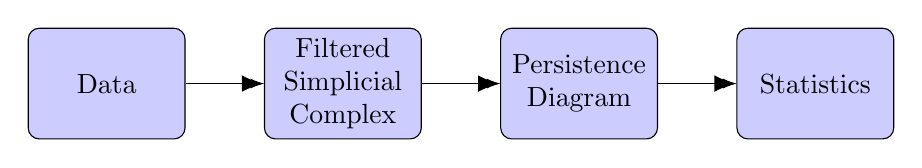
\begin{tikzpicture}[node distance = 2.5cm, auto, scale=0.8, decoration={
      markings,
      mark=at position 1 with {\arrow[scale=2,black]{latex}};
    }
  ]
   % Place nodes
    \node [block] (data) {Data};%Underling Probability Space
    \node [block, right of=data, node distance = 3cm] (simplex) {Filtered Simplicial Complex};
    \node [block, right of=simplex,node distance = 3cm] (pd) {Persistence Diagram};
    \node [block, right of=pd, node distance = 3cm] (stat) {Statistics};
   % Draw edges
    \path [line, postaction={decorate}] (data) -- (simplex);
    \path [line, postaction={decorate}] (simplex) -- (pd);
    \path [line, postaction={decorate}] (pd) -- (stat);
  \end{tikzpicture}
\end{frame}

\begin{frame}
  \frametitle{Simplicial Complexes}
  A {\em simplicial complex} is a combinatorial object, generalizing the notion of a graph. Each
  simplicial complex is built out of {\em simplices} of varying dimensions.

  \begin{center}
    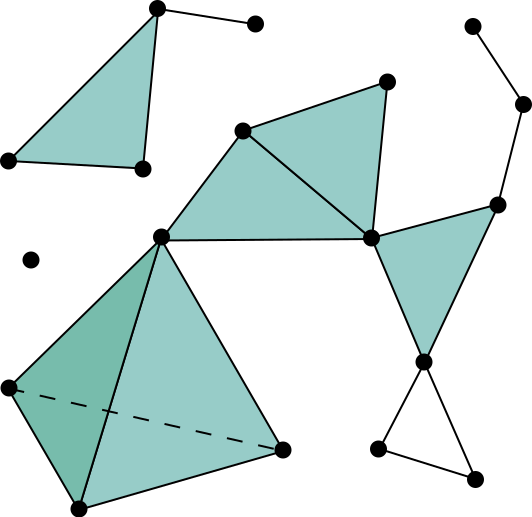
\includegraphics[scale=0.35]{Simplicial_complex_example.png}
  \end{center}
\end{frame}

\begin{frame}
  \frametitle{Betti numbers of simplicial complexes}
  \begin{align*}
    \beta_0 & =  \# \text{ of connected components}\\
    \beta_1 & =  \# \text{ of holes}\\
    \beta_2 & =  \# \text{ of voids}
  \end{align*}
  \begin{columns}
    \begin{column}{0.4\textwidth}
      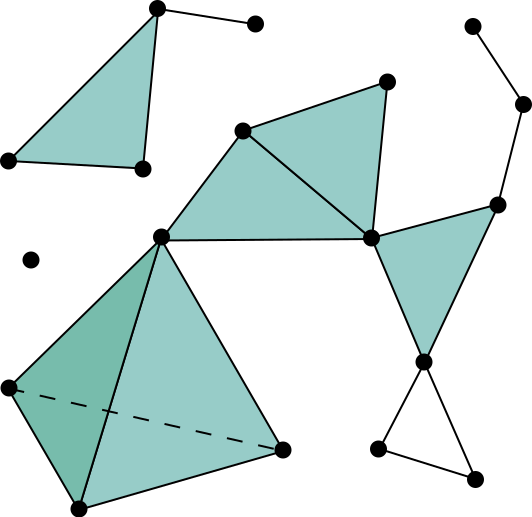
\includegraphics[height=45mm]{Simplicial_complex_example.png}
    \end{column}
    \begin{column}{0.2\textwidth}
      \begin{eqnarray*}
        \beta_0 & = & \visible<2>{3}\\
        \beta_1 & = & \visible<2>{1}\\
        \beta_2 & = & \visible<2>{1}
      \end{eqnarray*}
    \end{column}
  \end{columns}
  \bigskip
\end{frame}


\begin{frame} \frametitle{Homology of simplicial complexes}
  \begin{definition}
    Homology in degree $k$ is given by $k$-cycles modulo the $k$-boundaries.
  \end{definition}

\begin{center}
\definecolor{zzttqq}{rgb}{0.6,0.2,0}
\definecolor{qqqqff}{rgb}{0,0,1}
\begin{tikzpicture}[line cap=round,line join=round,x=1.0cm,y=1.0cm,scale=1.5]
% \draw[->,color=black] (-4.3,0) -- (7.5,0);
% \foreach \x in {-4,-3,-2,-1,1,2,3,4,5,6,7}
% \draw[shift={(\x,0)},color=black] (0pt,2pt) -- (0pt,-2pt) node[below] {\footnotesize $\x$};
% \draw[->,color=black] (0,-3.1) -- (0,6.3);
% \foreach \y in {-3,-2,-1,1,2,3,4,5,6}
% \draw[shift={(0,\y)},color=black] (2pt,0pt) -- (-2pt,0pt) node[left] {\footnotesize $\y$};
% \draw[color=black] (0pt,-10pt) node[right] {\footnotesize $0$};
% \clip(-4.3,-3.1) rectangle (7.5,6.3);
\fill[color=red,fill=red,fill opacity=0.2] (1,4.5) -- (2.1,5.3) -- (2.4,4.1) -- cycle;
\fill[color=red,fill=red,fill opacity=0.2] (1,4.5) -- (1,3) -- (2.4,4.1) -- cycle;
\fill[color=red,fill=red,fill opacity=0.2] (1,3) -- (1.8,2.2) -- (2.4,4.1) -- cycle;
\fill[color=red,fill=red,fill opacity=0.2] (1.8,2.2) -- (2.5,2.9) -- (2.4,4.1) -- cycle;
\fill[color=red,fill=red,fill opacity=0.2] (2.1,5.3) -- (3.7,4.9) -- (2.4,4.1) -- cycle;
\fill[color=red,fill=red,fill opacity=0.2] (3.7,4.9) -- (2.5,2.9) -- (2.4,4.1) -- cycle;
\fill[color=red,fill=red,fill opacity=0.2] (1.8,2.2) -- (3.1,2.2) -- (2.5,2.9) -- cycle;
\fill[color=red,fill=red,fill opacity=0.2] (3.1,2.2) -- (4,3) -- (5,2.3) -- cycle;
\fill[color=red,fill=red,fill opacity=0.2] (4,3) -- (4.8,3.2) -- (5,2.3) -- cycle;
\fill[color=red,fill=red,fill opacity=0.2] (5.5,4.7) -- (6.2,5.2) -- (6.3,3.9) -- cycle;
\fill[color=red,fill=red,fill opacity=0.2] (6.3,3.9) -- (6.2,2.8) -- (6.9,3.2) -- cycle;
\fill[color=red,fill=red,fill opacity=0.2] (3.7,4.9) -- (4.7,4.5) -- (4,3) -- cycle;
\fill[color=red,fill=red,fill opacity=0.2] (3.7,4.9) -- (5.5,4.7) -- (4.7,4.5) -- cycle;
\fill[color=red,fill=red,fill opacity=0.2] (4.7,4.5) -- (4.8,3.2) -- (4,3) -- cycle;
\fill[color=red,fill=red,fill opacity=0.2] (3.7,4.9) -- (3.4,3.5) -- (2.5,2.9) -- cycle;
\fill[color=red,fill=red,fill opacity=0.2] (3.7,4.9) -- (4,3) -- (3.4,3.5) -- cycle;
\fill[color=red,fill=red,fill opacity=0.2] (2.5,2.9) -- (3.2,2.9) -- (3.4,3.5) -- cycle;
\fill[color=red,fill=red,fill opacity=0.2] (3.2,2.9) -- (3.1,2.2) -- (2.5,2.9) -- cycle;
\fill[color=red,fill=red,fill opacity=0.2] (3.2,2.9) -- (4,3) -- (3.4,3.5) -- cycle;
\fill[color=red,fill=red,fill opacity=0.2] (3.2,2.9) -- (3.1,2.2) -- (4,3) -- cycle;
\draw [thick,color=red] (1,4.5)-- (2.1,5.3);
\draw [thick,color=red] (2.1,5.3)-- (2.4,4.1);
\draw [thick,color=red] (2.4,4.1)-- (1,4.5);
\draw [thick,color=red] (1,4.5)-- (1,3);
\draw [thick,color=red] (1,3)-- (2.4,4.1);
\draw [thick,color=red] (2.4,4.1)-- (1,4.5);
\draw [thick,color=red] (1,3)-- (1.8,2.2);
\draw [thick,color=red] (1.8,2.2)-- (2.4,4.1);
\draw [thick,color=red] (2.4,4.1)-- (1,3);
\draw [thick,color=red] (1.8,2.2)-- (2.5,2.9);
\draw [thick,color=red] (2.5,2.9)-- (2.4,4.1);
\draw [thick,color=red] (2.4,4.1)-- (1.8,2.2);
\draw [thick,color=red] (2.1,5.3)-- (3.7,4.9);
\draw [thick,color=red] (3.7,4.9)-- (2.4,4.1);
\draw [thick,color=red] (2.4,4.1)-- (2.1,5.3);
\draw [thick,color=red] (3.7,4.9)-- (2.5,2.9);
\draw [thick,color=red] (2.5,2.9)-- (2.4,4.1);
\draw [thick,color=red] (2.4,4.1)-- (3.7,4.9);
\draw [thick,color=red] (1.8,2.2)-- (3.1,2.2);
\draw [thick,color=red] (3.1,2.2)-- (2.5,2.9);
\draw [thick,color=red] (2.5,2.9)-- (1.8,2.2);
\draw [thick,color=red] (3.7,4.9)-- (4.7,4.5);
\draw [thick,color=red] (4.7,4.5)-- (5.5,4.7);
\draw [thick,color=red] (3.1,2.2)-- (4,3);
\draw [thick,color=red] (4,3)-- (5,2.3);
\draw [thick,color=red] (5,2.3)-- (3.1,2.2);
\draw [thick,color=red] (4,3)-- (4.8,3.2);
\draw [thick,color=red] (4.8,3.2)-- (5,2.3);
\draw [thick,color=red] (5,2.3)-- (4,3);
\draw [thick,color=red] (5.5,4.7)-- (6.2,5.2);
\draw [thick,color=red] (6.2,5.2)-- (6.3,3.9);
\draw [thick,color=red] (6.3,3.9)-- (5.5,4.7);
\draw [thick,color=red] (6.3,3.9)-- (6.2,2.8);
\draw [thick,color=red] (6.2,2.8)-- (6.9,3.2);
\draw [thick,color=red] (6.9,3.2)-- (6.3,3.9);
\draw [thick,color=red] (5,2.3)-- (6.2,2.8);
\draw [thick,color=red] (3.7,4.9)-- (4.7,4.5);
\draw [thick,color=red] (4.7,4.5)-- (4,3);
\draw [thick,color=red] (4,3)-- (3.7,4.9);
\draw [thick,color=red] (3.7,4.9)-- (5.5,4.7);
\draw [thick,color=red] (5.5,4.7)-- (4.7,4.5);
\draw [thick,color=red] (4.7,4.5)-- (3.7,4.9);
\draw [thick,color=red] (4.7,4.5)-- (4.8,3.2);
\draw [thick,color=red] (4.8,3.2)-- (4,3);
\draw [thick,color=red] (4,3)-- (4.7,4.5);
\draw [thick,color=red] (3.7,4.9)-- (3.4,3.5);
\draw [thick,color=red] (3.4,3.5)-- (2.5,2.9);
\draw [thick,color=red] (2.5,2.9)-- (3.7,4.9);
\draw [thick,color=red] (3.7,4.9)-- (4,3);
\draw [thick,color=red] (4,3)-- (3.4,3.5);
\draw [thick,color=red] (3.4,3.5)-- (3.7,4.9);
\draw [thick,color=red] (2.5,2.9)-- (3.2,2.9);
\draw [thick,color=red] (3.2,2.9)-- (3.4,3.5);
\draw [thick,color=red] (3.4,3.5)-- (2.5,2.9);
\draw [thick,color=red] (3.2,2.9)-- (3.1,2.2);
\draw [thick,color=red] (3.1,2.2)-- (2.5,2.9);
\draw [thick,color=red] (2.5,2.9)-- (3.2,2.9);
\draw [thick,color=red] (3.2,2.9)-- (4,3);
\draw [thick,color=red] (4,3)-- (3.4,3.5);
\draw [thick,color=red] (3.4,3.5)-- (3.2,2.9);
\draw [thick,color=red] (3.2,2.9)-- (3.1,2.2);
\draw [thick,color=red] (3.1,2.2)-- (4,3);
\draw [thick,color=red] (4,3)-- (3.2,2.9);
\begin{scriptsize}
\fill [color=qqqqff] (1,4.5) circle (1.5pt);
\fill [color=qqqqff] (2.1,5.3) circle (1.5pt);
\fill [color=qqqqff] (2.4,4.1) circle (1.5pt);
\fill [color=qqqqff] (1,3) circle (1.5pt);
\fill [color=qqqqff] (1.8,2.2) circle (1.5pt);
\fill [color=qqqqff] (2.5,2.9) circle (1.5pt);
\fill [color=qqqqff] (3.7,4.9) circle (1.5pt);
\fill [color=qqqqff] (3.1,2.2) circle (1.5pt);
\fill [color=qqqqff] (4.7,4.5) circle (1.5pt);
\fill [color=qqqqff] (5.5,4.7) circle (1.5pt);
\fill [color=qqqqff] (4,3) circle (1.5pt);
\fill [color=qqqqff] (5,2.3) circle (1.5pt);
\fill [color=qqqqff] (4.8,3.2) circle (1.5pt);
\fill [color=qqqqff] (6.2,5.2) circle (1.5pt);
\fill [color=qqqqff] (6.3,3.9) circle (1.5pt);
\fill [color=qqqqff] (6.2,2.8) circle (1.5pt);
\fill [color=qqqqff] (6.9,3.2) circle (1.5pt);
\fill [color=qqqqff] (3.4,3.5) circle (1.5pt);
\fill [color=qqqqff] (3.2,2.9) circle (1.5pt);
\end{scriptsize}
\uncover<2->{
\draw[color=blue,line width=1mm] (1,3) -- (2.4,4.1) -- (3.7,4.9) -- (4,3) -- (3.4,3.5) -- (3.2,2.9) -- (2.5,2.9) -- (1.8,2.2) -- cycle;
\draw[color=blue,line width=1mm] (4.7,4.5) -- (4.8,3.2) -- (5,2.3) -- (6.2,2.8) -- (6.9,3.2) -- (6.3,3.9) -- (5.5,4.7) -- cycle;
}
\end{tikzpicture}
\end{center}
\end{frame}


\begin{frame}
  \frametitle{Overview of TDA}
\centering
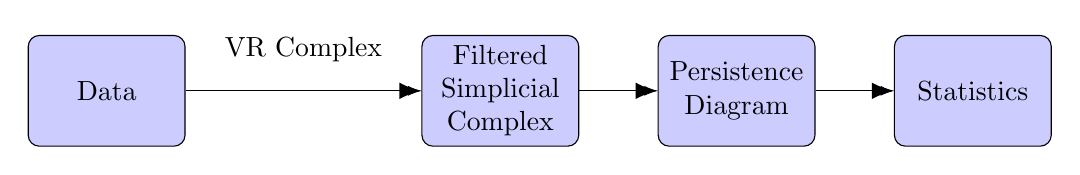
\begin{tikzpicture}[node distance = 2.5cm, auto, scale=0.8, decoration={
      markings,
      mark=at position 1 with {\arrow[scale=2,black]{latex}};
    }
  ]
   % Place nodes
    \node [block] (data) {Data};
    \node [block, right of=data, node distance = 5cm] (simplex) {Filtered Simplicial Complex};
    \node [block, right of=simplex,node distance = 3cm] (pd) {Persistence Diagram};
    \node [block, right of=pd, node distance = 3cm] (stat) {Statistics};
   % Draw edges
    \path [line, postaction={decorate}] (data) -- (simplex) 
    node [midway, label=above:VR Complex] {};
    \path [line, postaction={decorate}] (simplex) -- (pd);
    \path [line, postaction={decorate}] (pd) -- (stat);
  \end{tikzpicture}
\end{frame}

\begin{frame}
  \frametitle{Simplicial Complexes from Point data}
  \begin{block}{Definition}
    A {\em point cloud} $P$ is a finite metric space.
  \end{block}

  \begin{block}{Definition}
    The {\em Vietoris-Rips} complex of $P$ of parameter $i \in \R$ is the 
    simplicial complex with one $k$-simplex for every $k+1$ points with maximum 
    pairwise distance at most $i$.
  \end{block}

  couple pictures of this.
\end{frame}



\begin{frame}{Processing demo}
\end{frame}

\begin{frame}{TDA for Data Analysis}

\end{frame}
\end{document}
